\section{Musical scales and intervals}

\bi

\i A scale is basically a division of the octave 
into a succession of notes, in ascending or descending order.

\i The most common scales in Western music are
the {\em chromatic}, {\em diatonic}, and {\em pentatonic}
scales, consisting of 12, 7, and 5 intervals per octave, 
respectively.

\i In this section, we shall describe these scales and the most
common musical intervals.

\ei

%%%%%%%%%%%%%%%%%%%%%%%%%%%%%%%%%%%%%%%%%%%
\subsection{Chromatic scale}
\bi

\i A chromatic scale divides the octave into 
12 intervals called {\em semitones} or {\em half-steps}.
In {\em equal temperament} tuning (more about
this in a later section),
these intervals all have
the same size, corresponding to a frequency ratio of 
%
\be
2^{1/12} = 1.05946
\ee
%

\i Oftentimes it is more convenient to work in
term of {\em cents}, where a cent is the 
frequency interval corresponding to 1/100 of a semitone:
%
\be
2^{1/1200} = 1.000578
\ee
%

\i The human ear can distinguish frequencies
that differ by about 10 cents, which corresponds to
a frequency ratio of $2^{10/1200}=1.00579$,
or about a 0.5\% difference in frequency.
(We will discuss this in more detail in a later
section when we talk about {\em just noticeable
difference} for pitch.)

\i Figure~\ref{f:chromatic-scale-keyboard} shows the
corresponding notes in a chromatic scale on 
a piano keyboard:
%
\be
{\rm C}-{\rm C}^\sharp-{\rm D}-{\rm E}^\flat-{\rm E}-%
{\rm F}-{\rm F}^\sharp-{\rm G}-{\rm A}^\flat-{\rm A}-%
{\rm B}^\flat-{\rm B}-{\rm C}'
\nonumber
\ee
%
\begin{figure}[htbp]
\begin{center}
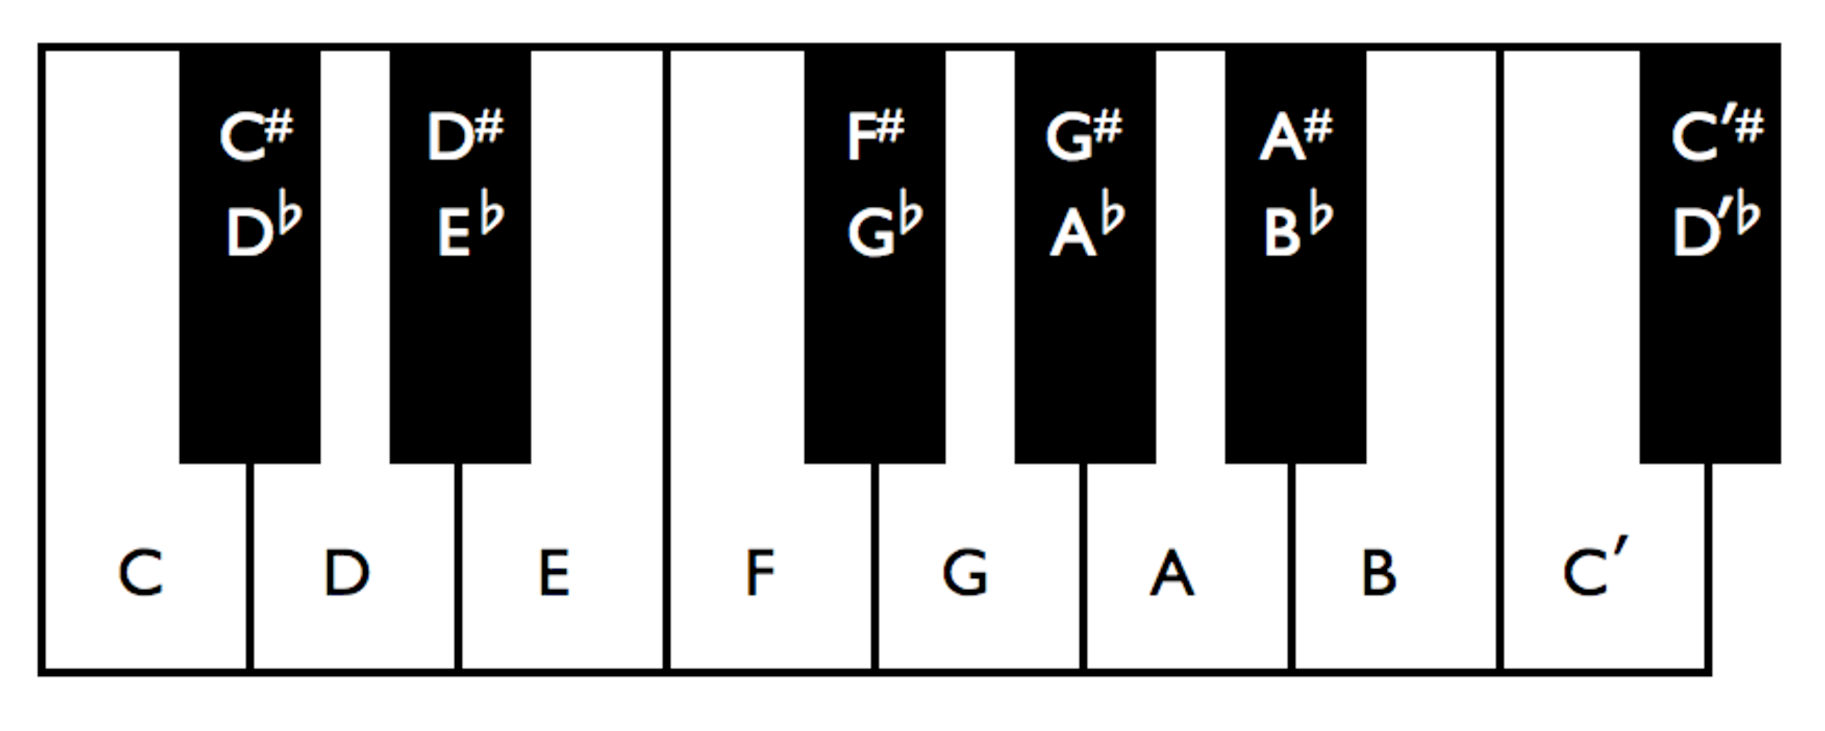
\includegraphics[width=.7\textwidth]{octave-keys}
\caption{Notes in a chromatic scale on a piano keyboard.}
\label{f:chromatic-scale-keyboard}
\end{center}
\end{figure}
%

\i On a piano, or any instrument tuned to
equal temperament, the sharps and flats are equal
to one another---e.g., C${}^\sharp$ and D${}^\flat$
are tuned to the same frequency.
These are called {\em enharmonic} notes.

\i A full piano keyboard, which has 88 keys 
ranging from A$_0$ to C$_8$, 
is a basically a logarithmic
frequency scale, with neighboring keys 
(white-black or white-white) corresponding
to a frequency interval of a semitone.

\i Figure~\ref{f:musical-staves-log-scale}
shows the correspondence between the treble and bass 
staves and their equal-tempered frequencies.
%
\begin{figure}[htbp]
\begin{center}
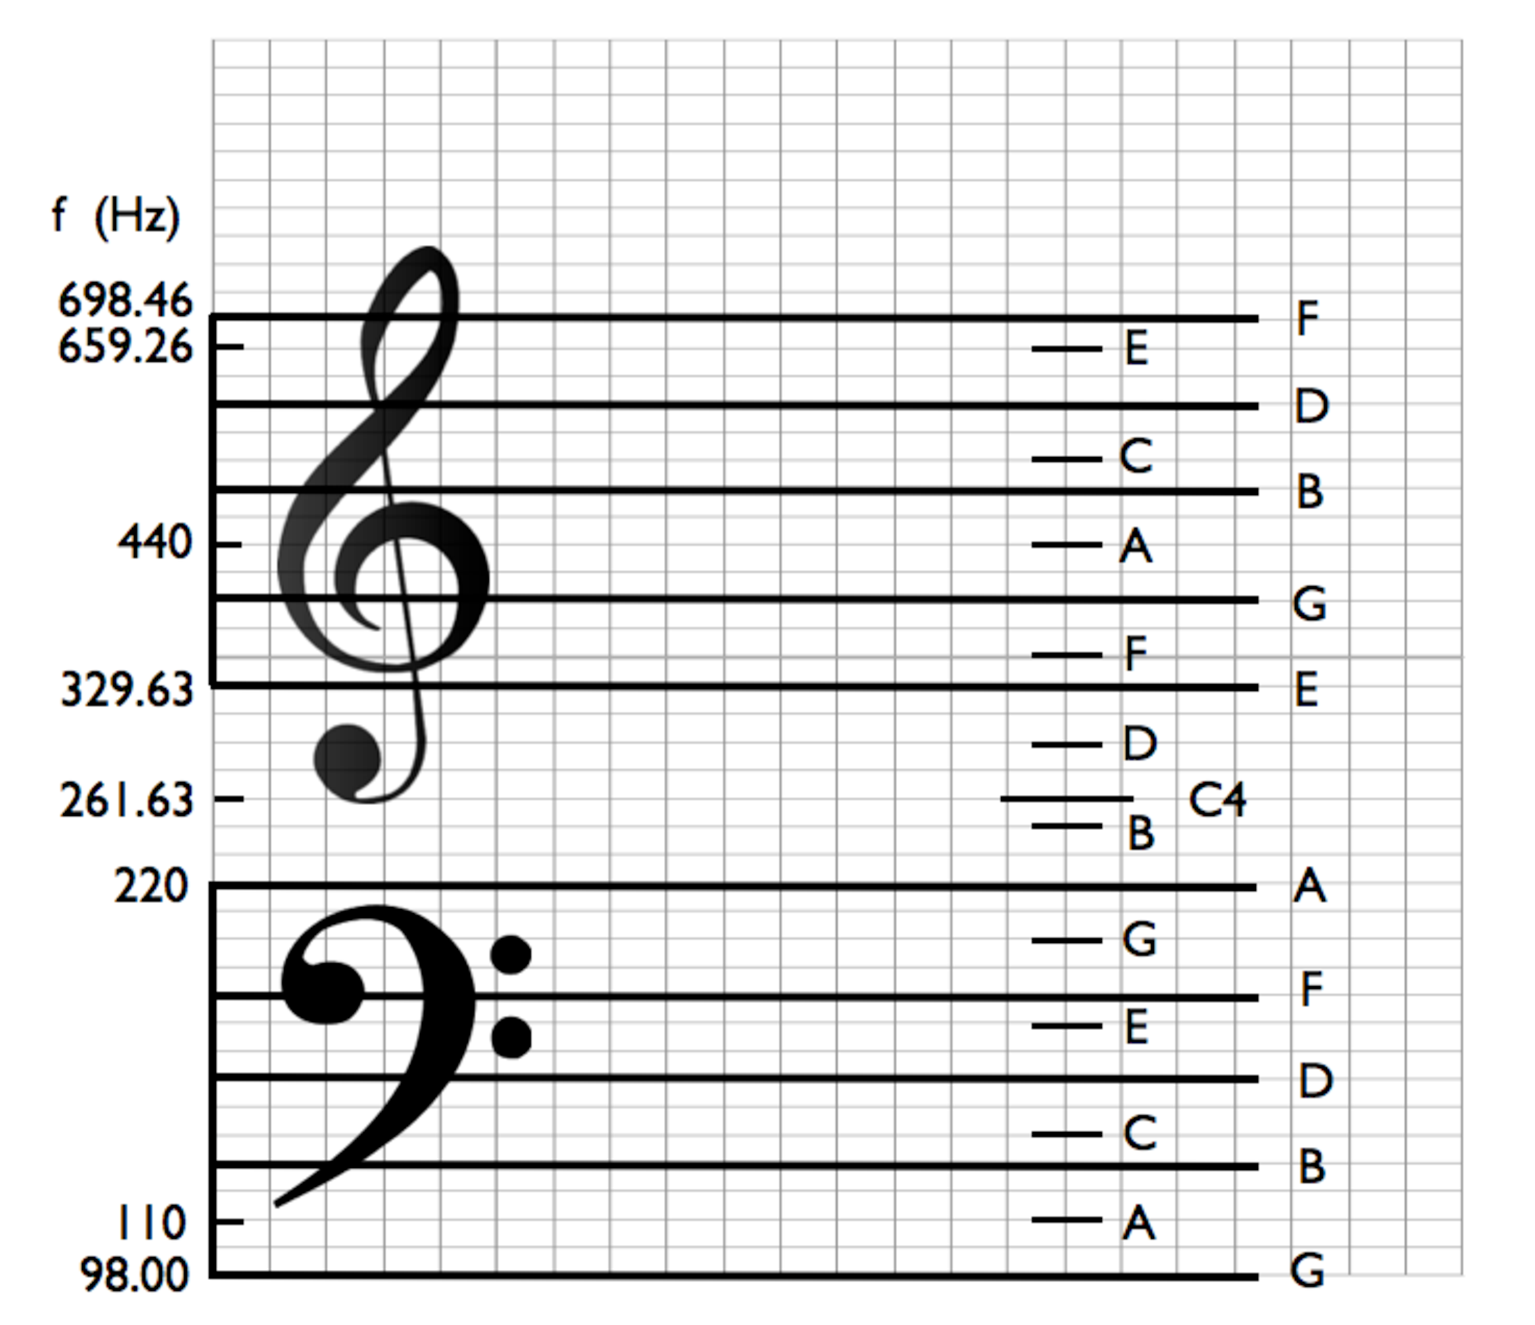
\includegraphics[width=.8\textwidth]{musical-staves-log-scale}
\caption{Correspondence between the treble and bass 
staves and their equal-tempered frequencies.}
\label{f:musical-staves-log-scale}
\end{center}
\end{figure}
%
This is another example of a logarithmic frequency
scale.

\i The staff lines are not equally-spaced
in this graph, since some divisions correspond to a 
minor third (three semitones), while other divisions
correspond to a major third (four semitones).

\ei
%%%%%%%%%%%%%%%%%%%%%%%%%%
\subsection{Diatonic scale}
\bi

\i A diatonic scale divides the octave into 
7 intervals consisting of both tones and semitones.
The order of tones and semitones 
defines the {\em major} and 
{\em minor} interval orders.

\i The diatonic major interval order is 
T-T-S-T-T-T-S (2-2-1-2-2-2-1).
This is the standard
%
\be
{\rm do-re-mi-fa-sol-la-ti-do}
\nonumber
\ee
%
interval order.

\i The diatonic minor interval order is
T-S-T-T-S-T-T (2-1-2-2-1-2-2).

\ei
%%%%%%%%%%%%%%%%%%%%%%%%%%%%%%%%%%%%%%%%%%%%%%%%%%%%%%%
\subsection{Musical intervals}
\bi

\i The most important musical interval is the
octave, corresponding to a frequency ratio of 
exactly 2.

\i Other common musical intervals are the 
fifth (C-G), 
fourth (C-F),
major third (C-E), and
minor third (C-E$^\flat$).

\i Table~\ref{t:musical-intervals} is a list of 
these and other musical intervals and their 
corresponding {\em just} and equal-tempered frequency ratios.
(We will describe the just temperament tuning system
in a later section.)

\begin{table}[htbp]
\begin{center}
\begin{tabular}{|l|c|c|c|c|c|}
\hline
Interval & \# semitones & Just freq ratio &
ET freq ratio & Difference (cents) & Example \\
\hline
Octave & 12 & $2:1=2.000$ & 2.000 & 0 & C-C$'$ \\
Fifth & 7 & $3:2=1.500$ & 1.498 & 2 & C-G \\
Fourth & 5 & $4:3=1.333$ & 1.335 & $-2$ & C-F, G-C$'$ \\
Major third & 4 & $5:4=1.250$ & 1.260 & $-14$ & C-E \\
Minor third & 3 & $6:5=1.200$ & 1.189 & 16 & C-E${}^\flat$, A-C$'$ \\
\hline
\end{tabular}
\caption{Common musical intervals and their corresponding
just and equal-tempered frequency ratios.}
\label{t:musical-intervals}
\end{center}
\end{table}

\i Mathematically, a musical interval corresponds to a 
{\em ratio} of frequencies.
Multiplication of frequency ratios corresponds
to addition of frequency intervals.

\i For example,
an octave equals a fifth plus a fourth,
and a fifth equals a major third plus a minor third:
%
\be
\frac{3}{2}\cdot \frac{4}{3} = \frac{2}{1}\,,
\qquad
\frac{5}{4}\cdot \frac{6}{5} = \frac{3}{2}
\ee
%

\ei
%%%%%%%%%%%%%%%%%%%%%%%%%%%%%%%%%%%%%%%%%%%%%%
\subsection{Harmonic series}
\bi

\i Notes in a harmonic series have frequencies that 
are integer multiples of some fundamental frequency:
$f_n= n f_1$, where $n=1,2,\cdots$.

\i Successive harmonics can be related to the musical 
intervals as shown in Figure~\ref{f:harmonics-keys},
where the fundamental frequency corresponds to A$_2$.
%
\begin{figure}[htbp]
\begin{center}
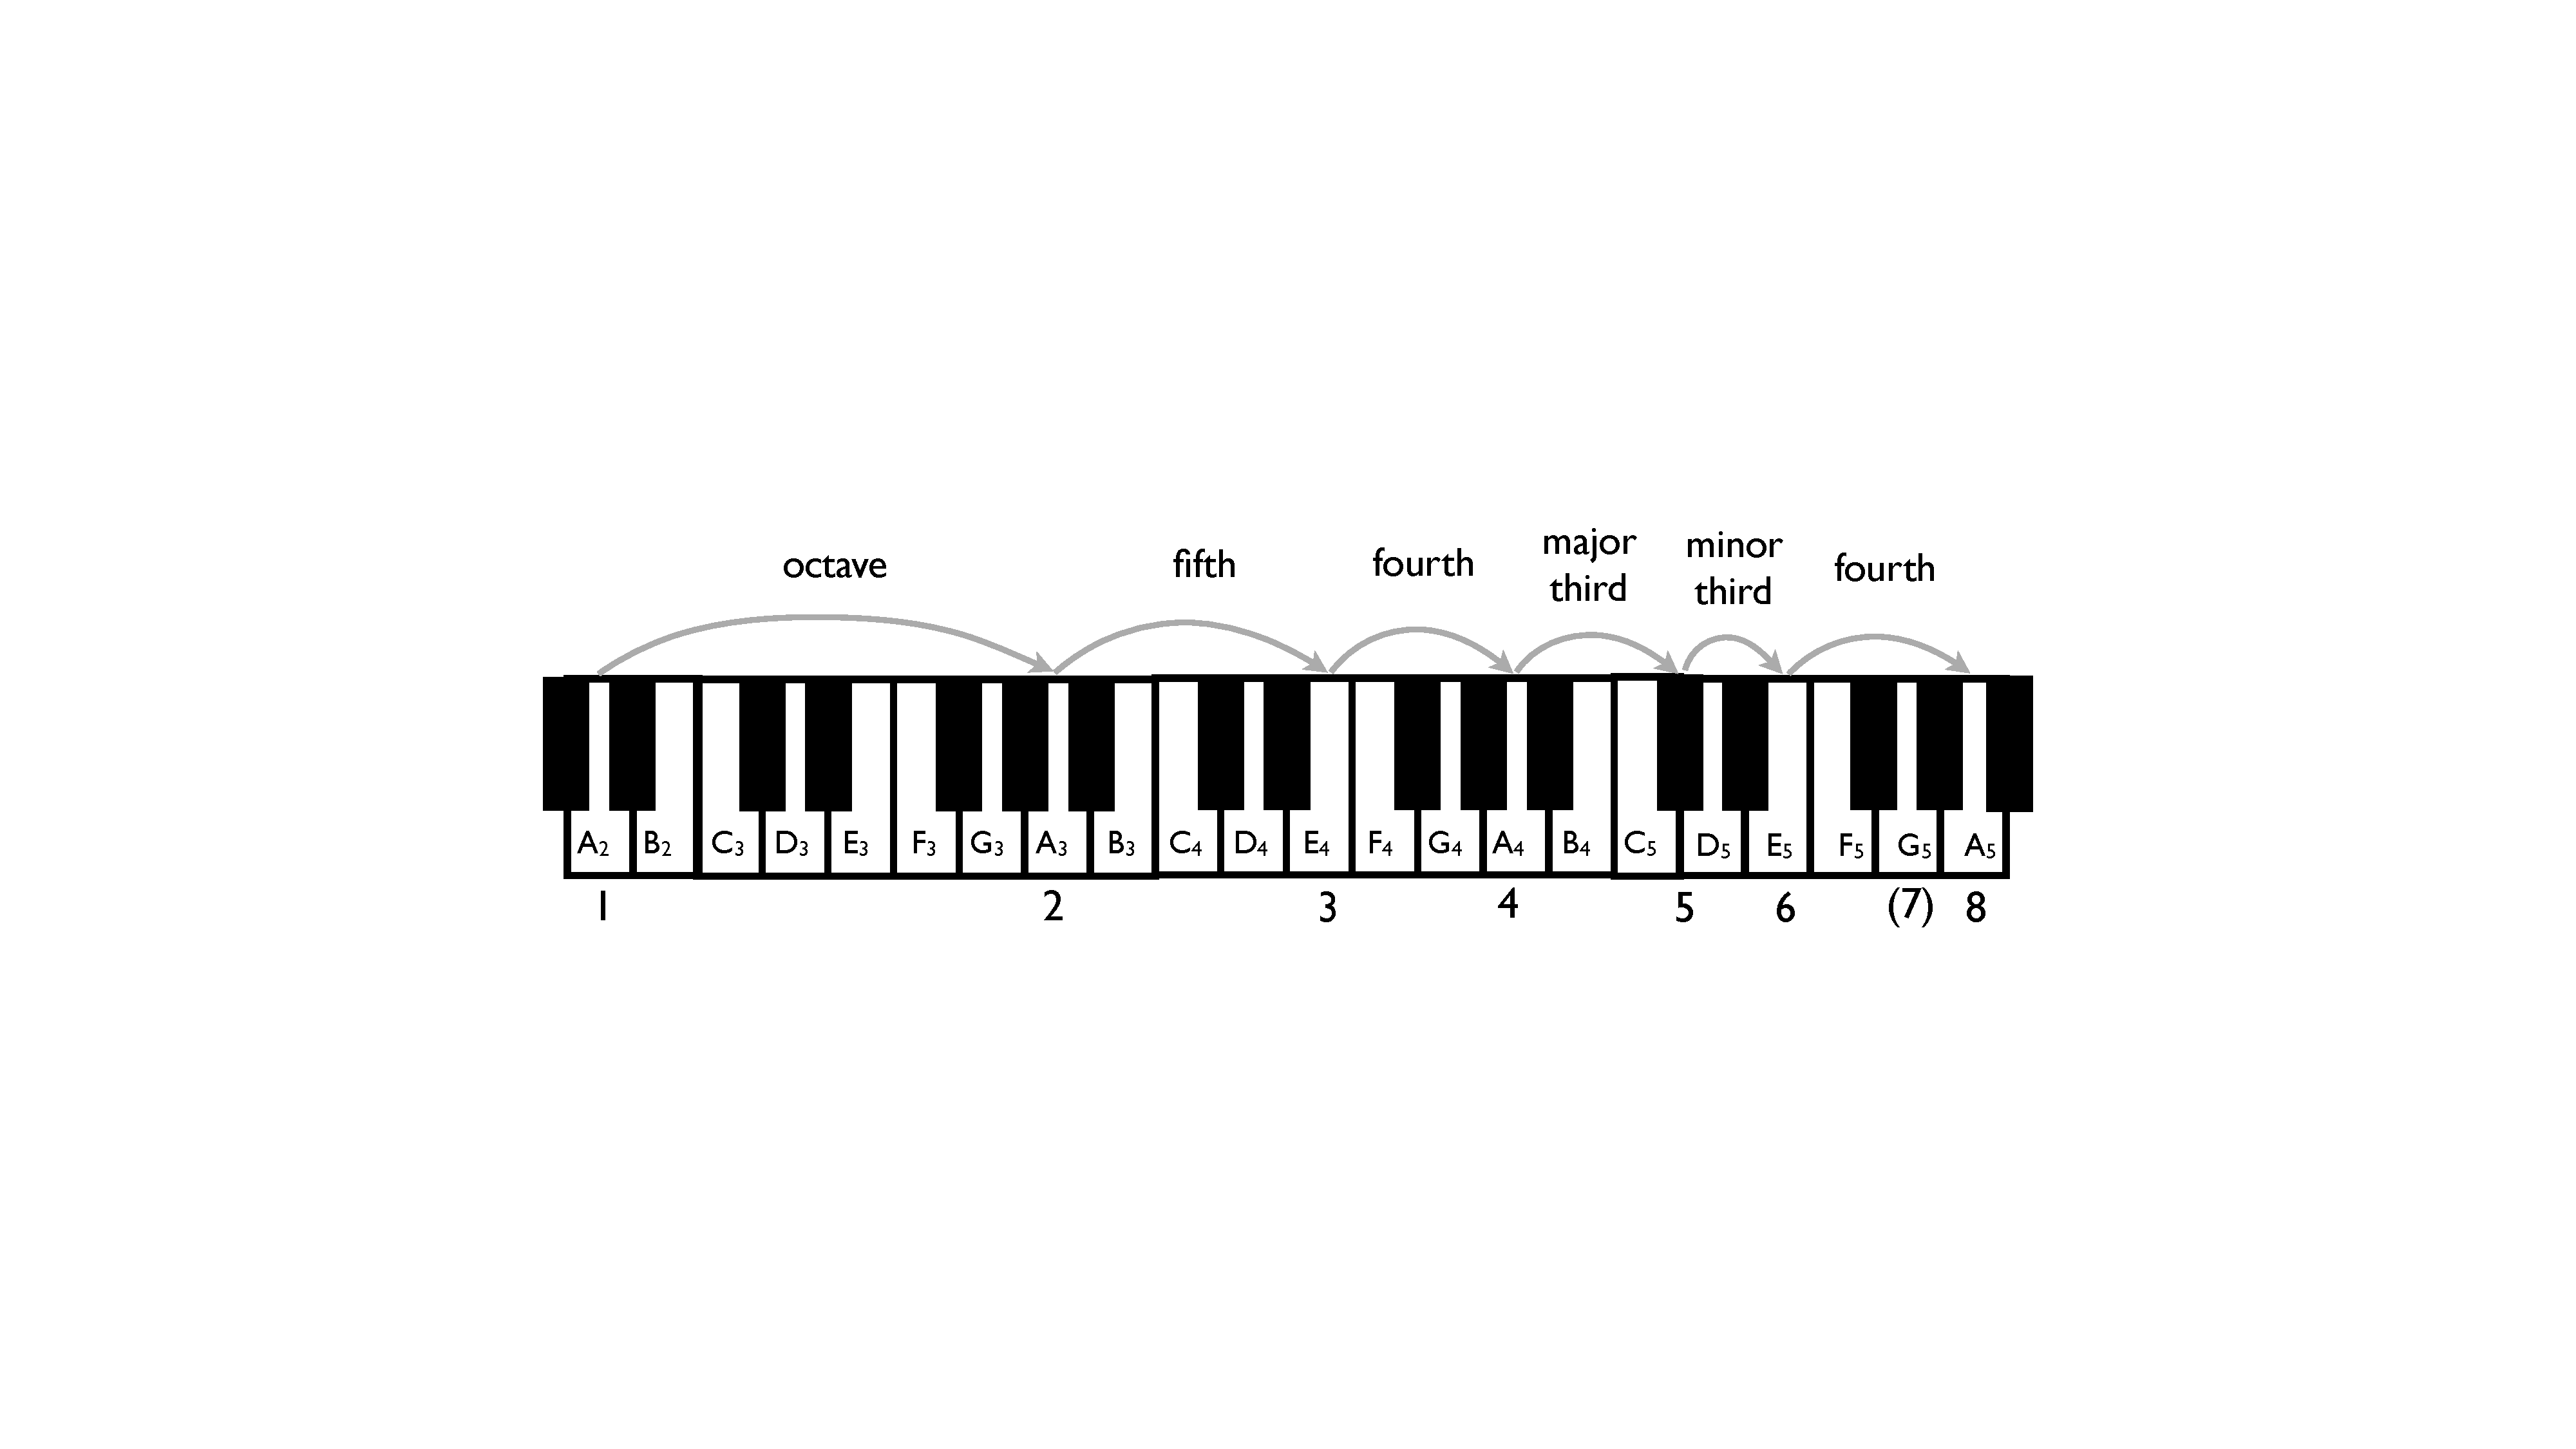
\includegraphics[width=\textwidth]{harmonics-keys}
\caption{Notes on a piano keyboard corresponding to
the first eight harmonics of A$_2$.}
\label{f:harmonics-keys}
\end{center}
\end{figure}
%

\i A comparison of the harmonic frequencies and
equal-tempered frequenices are given in 
Table~\ref{t:harmonics-ET}.
%
\begin{table}[htbp]
\begin{center}
\begin{tabular}{|c|c|c|c|c|}
\hline
Harmonic & Exact freq (Hz) & Equal-tempered freq (Hz) 
& Difference (cents) & Piano note \\ 
\hline
1 & 110 & 110.00 & 0 & A$_2$ \\
2 & 220 & 220.00 & 0 & A$_3$ \\
3 & 330 & 329.63 & 2 & E$_4$ \\
4 & 440 & 440.00 & 0 & A$_4$ \\
5 & 550 & 554.37 & $-14$ & C$_5^\sharp$ \\
6 & 660 & 659.26 & 2 & E$_5$ \\
7 & 770 & 783.99 & $-31$ & G$_5$ \\
8 & 880 & 880.00 & 0 & A$_5$ \\
\hline
\end{tabular}
\caption{Relation between harmonic frequencies
and equal-tempered frequencies.}
\label{t:harmonics-ET}
\end{center}
\end{table}

\i Note that the largest discrepancy in equal temperament
tuning is for the 7th harmonic.

\ei
%%%%%%%%%%%%%%%%%%%%%%%%%%%%%%%%%%%%%%%%%%%%%%%%
\subsection{Chords}
\bi

\i Chords: There are three major chords (triads) 
having just frequency ratios 4:5:6:
%
\be
{\rm C-E-G}\,,
\quad
{\rm F-A-C}\,,
\quad
{\rm G-B-D}
\nonumber
\ee
%
These three notes correspond to a major third followed by a minor third.

\i There are two minor chords (triads) 
having just frequency ratios 10:12:15:
%
\be
{\rm E-G-B}\,,
\quad
{\rm A-C-E}
\nonumber
\ee
%
These three notes correspond to a minor third followed by a major third.

\ei
%%%%%%%%%%%%%%%%%%%%%%%%%%%%%%%%%%%%%%%%%%%%%%%%
\subsection{Circle of fifths}
\bi

\i A useful construct is the so-called {\em circle of fifths}
shown in Figure~\ref{f:circle-of-fifths}.

\begin{figure}[htbp]
\begin{center}
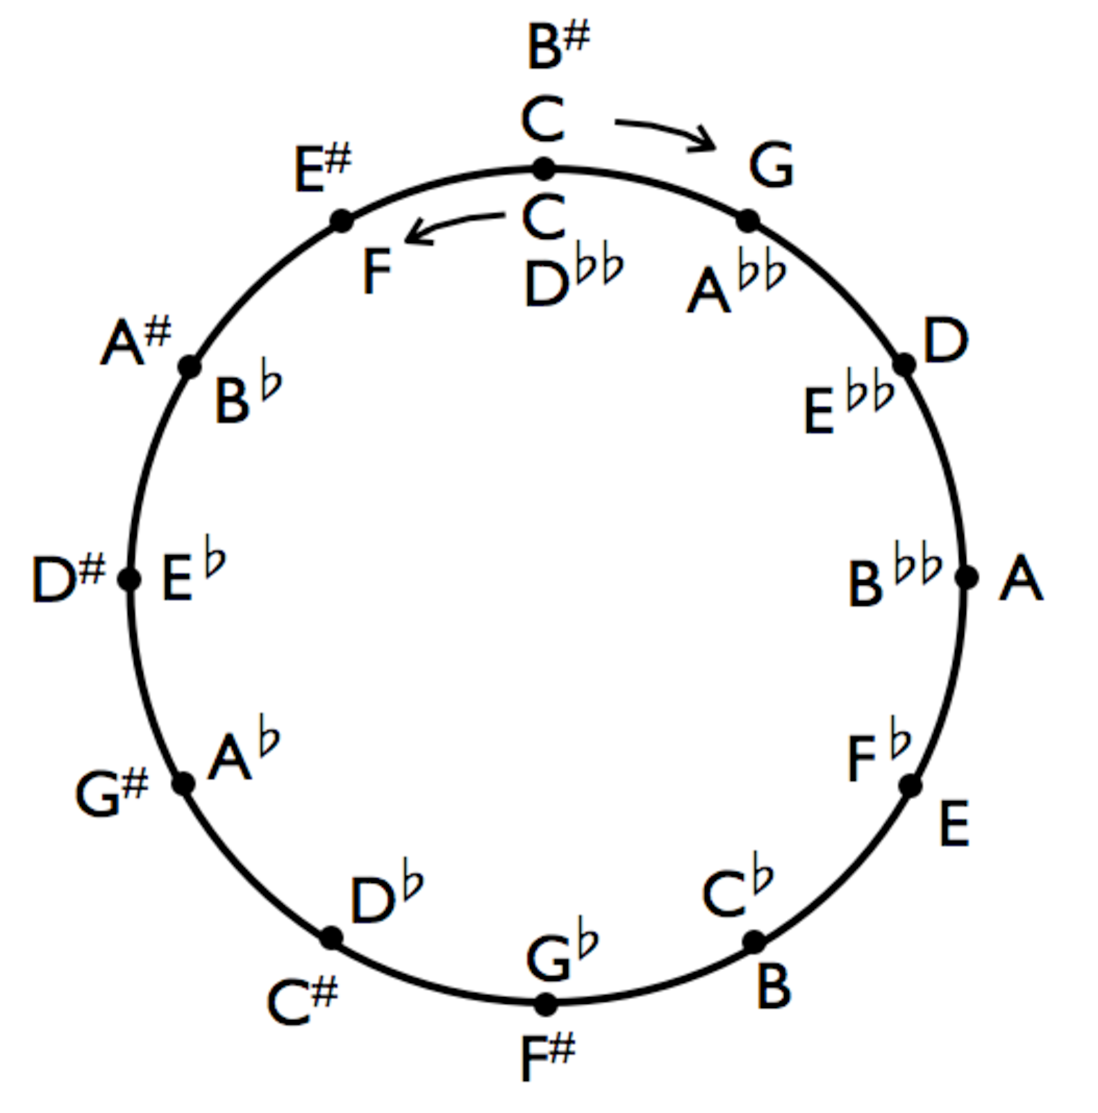
\includegraphics[width=.4\textwidth]{circle-of-fifths}
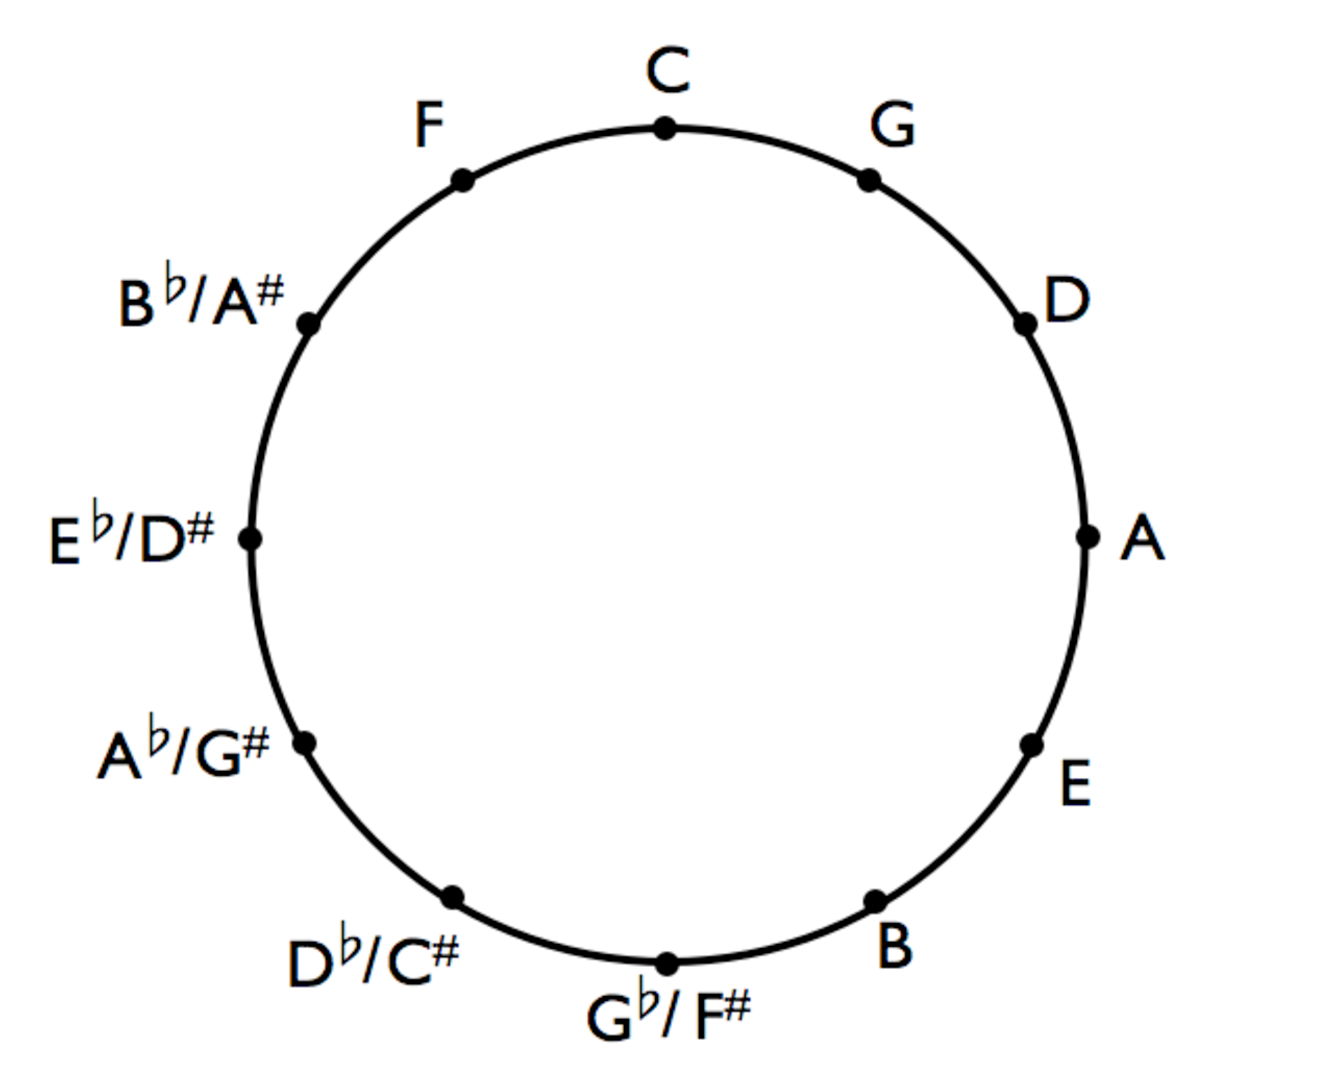
\includegraphics[width=.5\textwidth]{circle-of-fifths-simple}
\caption{Circle of fifths.
Left panel: General circle of fifths.
Right panel: Simplified circle of fifths for equal temperament tuning.}
\label{f:circle-of-fifths}
\end{center}
\end{figure}

\i Successive notes on the circle are separated by a musical fifth.

\i In equal temperament, the notes next to one another have the 
same frequency; 
this is not the case for other tuning systems such as Pythagorean
or just temperament, as we shall see in a later
section.
For these other tuning systems, the circle of fifths does {\em not}
close.

\ei
%%%%%%%%%%%%%%%%%%%%%%%%%
\subsection{Major and minor key signatures}
\bi

\i For example, the C-major and C-minor diatonic scales are:
\be
{\rm C-D-E-F-G-A-B}
\nonumber
\ee
% 
and
%
\be
{\rm C-D-E}^\flat{\rm -F-G-G}^\sharp{\rm -A}^\sharp
\nonumber
\ee

\i The notes in the G-major scale are the same as for C-major 
except for F$^\sharp$:
%
\be
{\rm G-A-B-C-D-E-F}^\sharp
\nonumber
\ee
% 

\i The notes in the F-major scale are the same as for C-major 
except for B$^\flat$:
%
\be
{\rm F-G-A-B}^\flat{\rm -C-D-E}
\nonumber
\ee
% 

\i Note that the A-minor scale is
%
\be
{\rm A-B-C-D-E-F-G}
\nonumber
\ee
% 
so the notes are {\em exactly} the same as for C-major.
But because the tonic (and tonal interval order) are 
different for these two scales, they sound differently.

\ei
%%%%%%%%%%%%%%%%%%%%%%%%%%%%%%%%%%%%%%%%%%%
\subsection{Pentatonic scale}
\bi

\i A pentatonic scale is probably the oldest 
division of the octave.
It was developed independently in many different cultures.

\i A pentatonic scale divides the octave into
5 intervals (3 intervals are whole tones and
2 intervals are three semitones wide).

\i Examples of pentatonic scales in major interval
order are
%
\be
{\rm C-D-E-G-A} 
\ee
%
and
%
\be
{\rm F{}^\sharp-G{}^\sharp-A{}^\sharp-C{}^\sharp-D{}^\sharp}
\ee
%
which are just the black keys on a piano.

\item
The pentatonic scale also has minor
and various modal inteval orders.
The major interval order is: 2-2-3-2-3.
The minor interval order is: 3-2-2-3-2.

\i A pentatonic scale can be constructed from 
just fifths and the octave 
(or, equivalently, from just fifths and fourths)
as a subset of Pythagorean temperament (see
next section).

\i A guitar (or any 6-string instrument) can be tuned 
to a pentatonic scale {\em using only the guitar to do
the tuning} as described below:

[To play a note {\em an octave above} an open note, touch the 
string at its half-way point (12th fret on a guitar) 
as you pluck it with your other hand.
Similarly, to play a note {\em a fifth above} an open note, 
touch the string at its one-third point (7th fret on a guitar)
as you pluck it with your other hand.]

Instructions (tuning order: string 6 (top), 1 (bottom), 3, 5, 2, 4):

- Adjust the tension of string 6 
to any value that gives it a nice sound (let us assume it's a C)

- Tune the open note of string 1 
to the note an octave above string 6 (then string 1 will be C$'$)

- Tune the open note of string 3 to the note 
a fifth above string 6 (then string 3 will be G)

- Tune the note an octave above string 5 to the note
a fifth above string 3 (then string 5 will be D)

- Tune the open note of string 2 to the note 
a fifth above string 5 (then string 2 will be A)

- Tune the note an octave above string 4 to the note
a fifth above string 2 (then string 4 will be E)

The result is the guitar tuned to the pentatonic
scale in major interval order 2-2-3-2-3;
for this example, it is the key of C corresponding to 
the notes C-D-E-G-A-C$'$.

\i \demo
Examples of music played using a pentatonic scale are
``Amazing Grace," 
``Auld Lang Syne," 
``My Girl" (by the Temptations), and
Etude Op.10 No.5 (Black Keys) by Chopin.

Watch YouTube video of pianist Vladimir Horowitz playing 
Chopin's etude \\
(http://www.youtube.com/watch?v=jaMA8LWW3C0).

\subsection{Normal tuning of a violin and a guitar}

\i A violin has four strings.  
They are normally tuned to
\be
{\rm G_3 - D_4 - A_4 - E_5}
\ee
which are all separated by fifths.

\i A guitar has six strings.
They are normally tuned to
\be
{\rm E_2 - A_2 - D_3 - G_3 - B_3 - E_4}
\ee
which are all separated by fourths 
except for G$_3$ to B$_3$, which is separated by a 
major third.

\i Note that using perfect fourths (ratio 4:3) and
a perfect major third (ratio 5:4), the notes E2 and
E4 are not {\em exactly} two octaves apart, since
%
\be
\frac{4}{3}\cdot
\frac{4}{3}\cdot
\frac{4}{3}\cdot
\frac{5}{4}\cdot
\frac{4}{3}
= \frac{80}{81}\cdot 4
\ee
%
which is slightly less than 4.

\i Slight discrepancies, such as this, were ultimately 
the reason for introducing the equal temperament (ET) tuning 
system (more about this later). 
The product of four equal-tempered fourths and an 
equal-tempered major third equals two octaves exactly.

\ei
